
\chapter{Introduction to Numerical Methods relevant to Thermodynamics}\label{Appendix_NumMethods}

%%%
%%% SECTION
%%%
\section{Linear Interpolation}\label{LinearInterpolation}\index{Linear interpolation}

Given a continuous and unknown function $f(x)$, defined at a set of points  $x_{1} < \cdots < x_{i} < \cdots < x_{N}$. Interpolation is the process of determining a polynomial expression to calculate the pair $\left[x_{k}, f\left(x_{k}\right)\right]$ based on neighbours discrete coordinates $\left\{\left[x_{1},f\left(x_{1}\right)\right], \cdots, \left[x_{N},f\left(x_{N}\right)\right]\right\}$. 

Consider a set of discrete data points,

  \begin{tabular}{c | c }
      {\bf x}   & {\bf f(x)} \\
       \hline
         $x_{1}$ &  $y_{1}$ \\
         $x_{2}$ &  $y_{2}$ \\
         $x_{3}$ &  $y_{3}$ \\
         $x_{4}$ &  $y_{4}$ \\
  \end{tabular}
that are a subset of a continuous and smooth function $y=f(x)$ (Fig.~\ref{Appendix:Fig:Interpolation}). Polynomials can be generated to represent this functions, a high-order polynomial can more accurately fit the points than a low-order one.   

     \begin{figure}\label{Appendix:Fig:Interpolation}%
        \begin{center}
          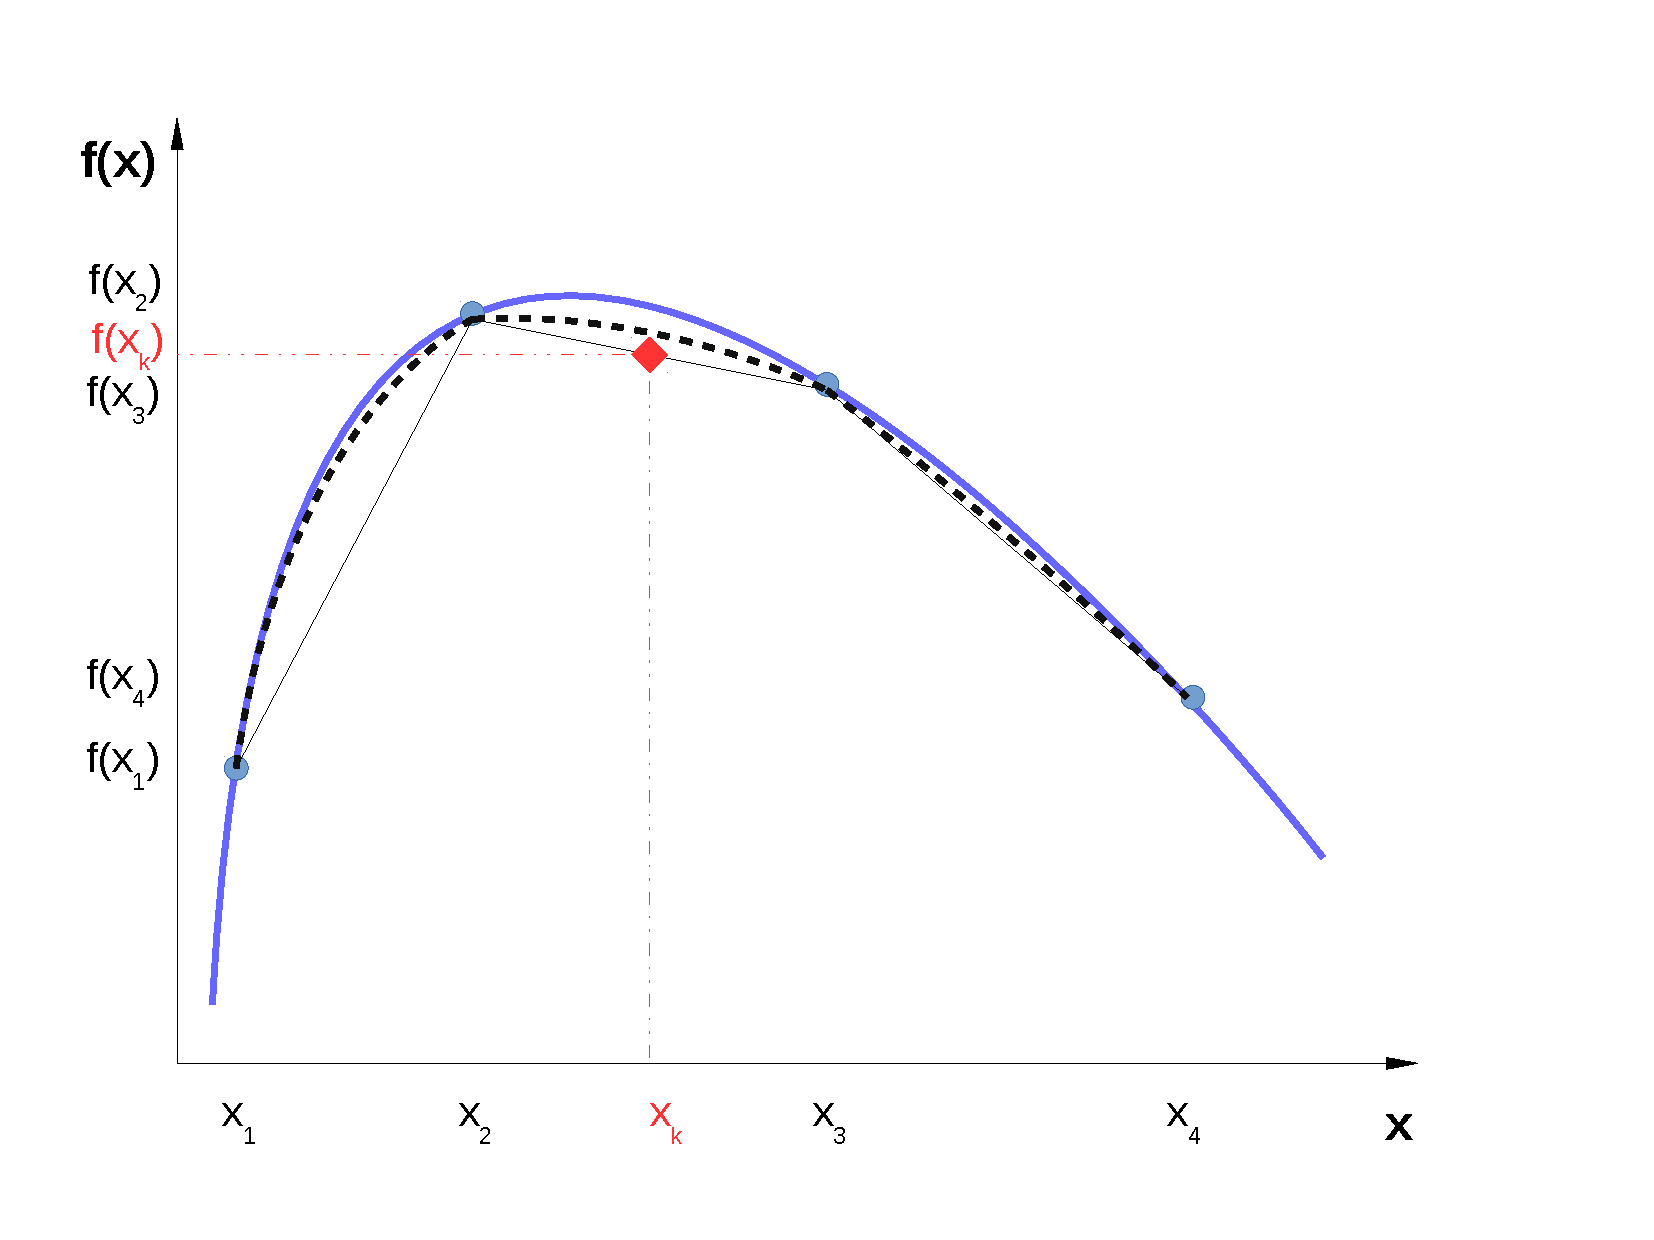
\includegraphics[width=\columnwidth,clip]{./Pics/Interpolation}
           \caption{Smooth function $f(x)$ (solid blue line) may be more accurately interpolated by a high-order polynomial (black dotted line) than by a low-order polynomial (solid black line).} 
        \end{center}
      \end{figure}


%%%
%%% SECTION
%%%
\section{Root Finder}
